% 2006 湖北理科第18题：源图所示正方体及上底面对角线；点 P 未画在源图中。
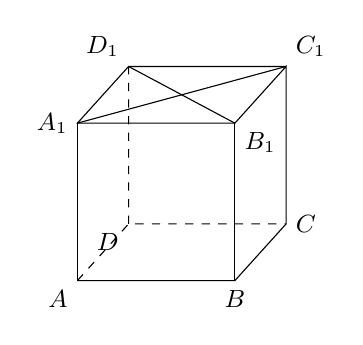
\begin{tikzpicture}[x=1cm, y=1cm, font=\small]
  \coordinate (A)  at (0,0);
  \coordinate (B)  at (2,0);
  \coordinate (C)  at (2.65,0.72);
  \coordinate (D)  at (0.65,0.72);
  \coordinate (A1) at (0,2);
  \coordinate (B1) at (2,2);
  \coordinate (C1) at (2.65,2.72);
  \coordinate (D1) at (0.65,2.72);

  % 可见棱
  \draw (A) -- (B) -- (C) -- (C1) -- (B1) -- (A1) -- (D1) -- (C1);
  \draw (A) -- (A1);
  \draw (B) -- (B1);
  % 源图中的隐藏棱
  \draw[dashed] (A) -- (D) -- (C) (D) -- (D1);
  % 顶面两条对角线
  \draw (A1) -- (C1);
  \draw (D1) -- (B1);

  \node[below left] at (A) {$A$};
  \node[below] at (B) {$B$};
  \node[right] at (C) {$C$};
  \node[below left] at (D) {$D$};
  \node[left] at (A1) {$A_1$};
  \node[below right] at (B1) {$B_1$};
  \node[above right] at (C1) {$C_1$};
  \node[above left] at (D1) {$D_1$};
\end{tikzpicture}
